\documentclass{beamer}

\usepackage{préambule}

\begin{document}

\begin{frame}
	Un jeu de cartes classiques comporte 52 cartes.

	\begin{center}
		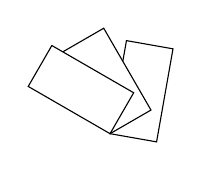
\begin{tikzpicture}[scale=0.6]
			\draw[fill=white,rotate=-10] (0,0) -- ++(1,0) -- ++(0,2) -- ++(-1,0) -- cycle;
			\draw[fill=white,rotate=30] (0,0) -- ++(1,0) -- ++(0,2) -- ++(-1,0) -- cycle;
			\draw[fill=white,rotate=60] (0,0) -- ++(1,0) -- ++(0,2) -- ++(-1,0) -- cycle;
		\end{tikzpicture}
	\end{center}

	On tire une carte au hasard dans le jeu.

	\begin{itemize}
		\item<2-> Quelle est la probabilité que cette carte soit le $5$ de pique ?
		\item<3-> Quelle est la probabilité que la carte soit du trèfle ?
			% Une issue
		\item<4-> « La carte est le cinq de pique » est appellée une ................
			% Un évènement
		\item<5-> « La carte est du trèfle » est appellée un .....................

			\visible<6->{On peut lui donner un nom, par exemple $T$ (comme $T$rèfle)}
		\item<7-> La probabilité que la carte soit du trèfle est alors notée .........
	\end{itemize}
\end{frame}

\end{document}